% !TEX root = reply_letter.tex
\section*{Response to 2nd Referee's Comments}
We would like to thank the Referee for his/her constructive comments, which have allowed us to considerably improve our paper. The main differences of the new version of the manuscript compared to the previous one can be found in Sections~5 and 6, Web Appendix A.2, C and D. In addition, changes regarding the specific comments have been made throughout the text.

You may find below our responses to the specific issues raised.

\subsection*{Major Concerns Shared by the 2nd Referee}
\begin{enumerate}
    \item [1.] \underline{Heavier tailed negative residuals in the quantile-quantile plot.}

    We would like to thank the Referee for motivating us to check the model fit. As the Referee noted, the quantile-quantile plot for the residuals from the original model (left panel of Figure ) shows heavy tailed negative residuals. Following the suggestion of the Referee we transformed the longitudinal outcome using a $\log_2 (\mbox{PSA}+0.1)$ transformation instead of the original $\log_2 (\mbox{PSA})$ transformation. In addition, we also tried $\log_2 (\mbox{PSA}+1)$ transformation \citep{lin2000latent,pearson1994mixed}. The resulting quantile-quantile plots of the residuals in shown in Figure \ref{fig : qqplot_various_log_transform_t3}. Since the residuals from the model with $\log_2(\mbox{PSA} + 1)$ transformation met the assumptions best, we use it in the revised version of the manuscript. The corresponding longitudinal sub-model of the joint model we fit is given by:
    \begin{equation}
    \label{eq : long_model_prias_ref2}
    \begin{aligned}
\log_2 (\mbox{PSA}_i + 1)(t) &= \beta_0 + \beta_1 (\mbox{Age}_i-70) + \beta_2 (\mbox{Age}_i-70)^2 + \sum_{k=1}^4 \beta_{k+2} B_k(t,\mathcal{K})\\ 
&+  b_{i0} + b_{i1} B_7(t, 0.1) + b_{i2} B_8(t, 0.1) +
\varepsilon_i(t),
\end{aligned}
\end{equation}
    where the error $\varepsilon_i(t)$ is assumed to be t-distributed with three degrees of freedom and scale $\sigma$.

    \begin{figure}[!htb]
    \centerline{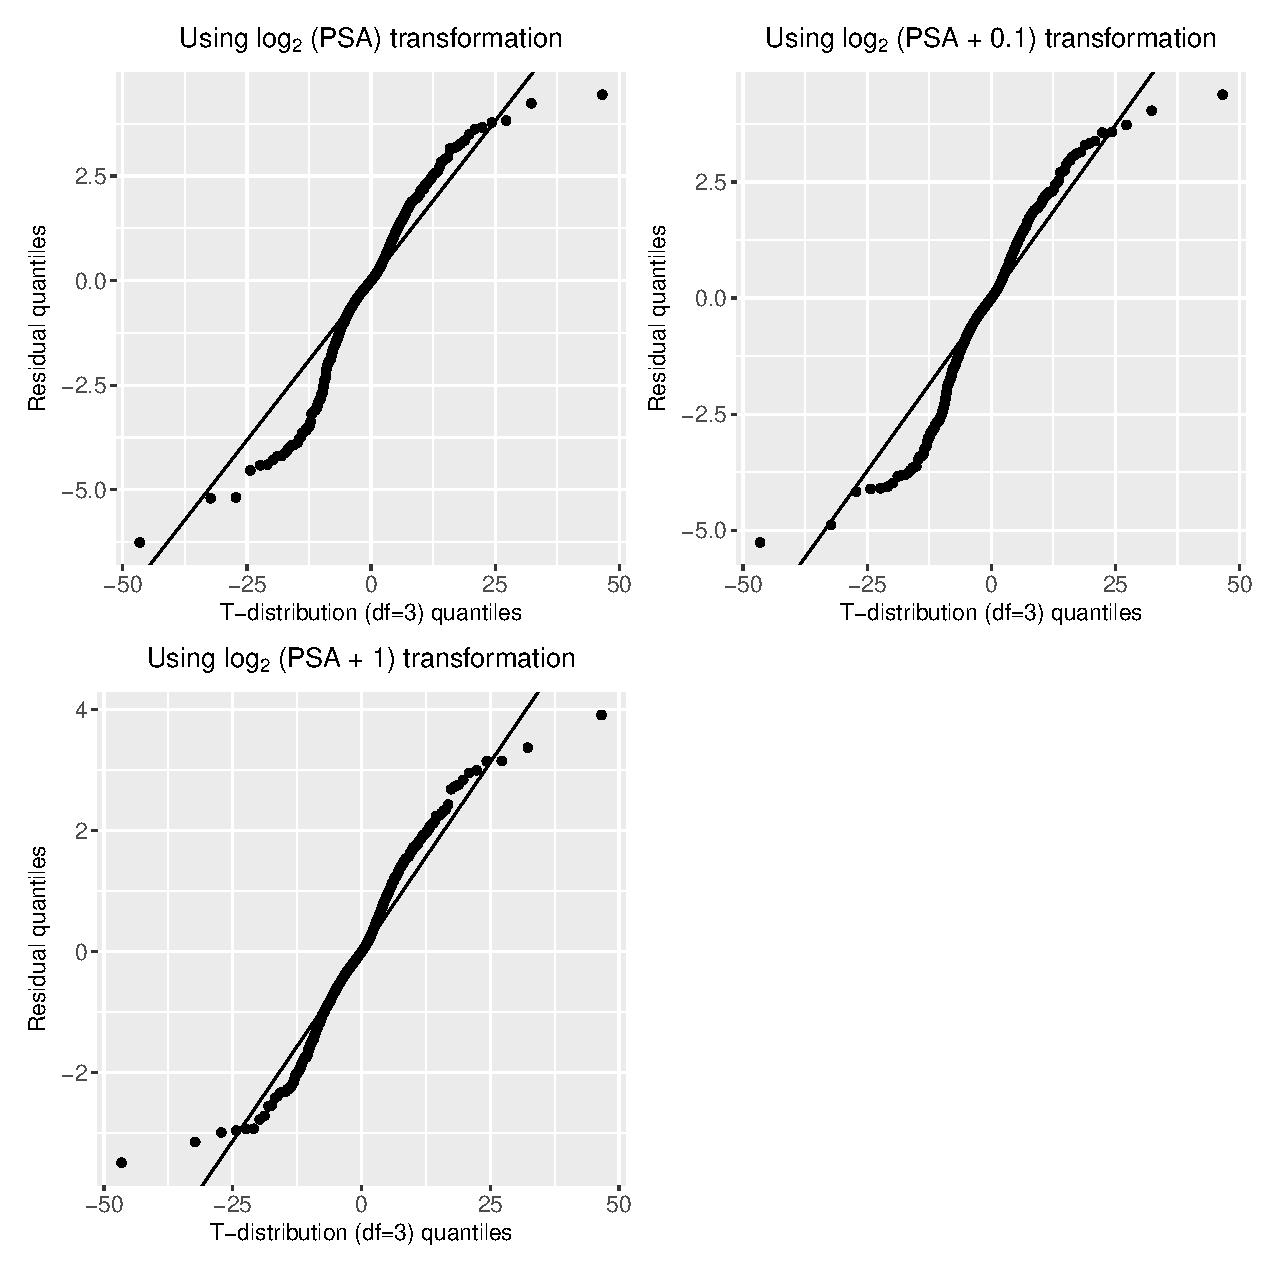
\includegraphics[width=\columnwidth]{../images/model_fit/qqplot_various_log_transform_t3.eps}}
    \caption{Quantile-quantile plots of subject specific residuals obtained from joint models with $\log_2 (\mbox{PSA})$, $\log_2(\mbox{PSA}+0.1)$, and $\log_2(\mbox{PSA}+1)$ transformed longitudinal outcome, and an assumption of t-distributed (df=3) errors, fitted to the PRIAS data set.}
    \label{fig : qqplot_various_log_transform_t3}
    \end{figure}

    
\end{enumerate}

\subsection*{Minor Concerns Shared by the 2nd Referee}

\begin{enumerate}
    \item[1.] \underline{More informative captions for tables and graphs.}

    We have now updated the captions of tables and graphs in the revised manuscript. How??????
    
    \item[2.] \underline{Missing subscript $i$ in Equation 7 of the original manuscript.}

    We thank the Referee for noticing this error. Equation (\ref{eq : long_model_prias_ref2}) in this reply letter shows the new equation that we use in the revised version of the manuscript.

\end{enumerate}

